\documentclass[conference]{IEEEtran}

\usepackage{cite}
\usepackage{amsmath,amssymb,amsfonts}
\usepackage{algorithmic}
\usepackage{graphicx}
\usepackage{textcomp}
\usepackage{xcolor}
\usepackage{booktabs}
\usepackage{multirow}
\usepackage{hyperref}
\usepackage{float}
\usepackage{listings}
\usepackage[utf8]{inputenc}
\usepackage{algorithm}

\def\BibTeX{{\rm B\kern-.05em{\sc i\kern-.025em b}\kern-.08em
    T\kern-.1667em\lower.7ex\hbox{E}\kern-.125emX}}

\lstset{
  basicstyle=\ttfamily\footnotesize,
  breaklines=true,
  frame=single,
  captionpos=b,
  tabsize=2,
  language=Python,
  keywordstyle=\color{blue},
  stringstyle=\color{red},
  commentstyle=\color{green!60!black},
  numbers=left,
  numberstyle=\tiny\color{gray}
}

\begin{document}

\title{A Multi-Agent AI System for Cash Flow Forecasting and Credit Intelligence in Indian SMEs}

\author{
\IEEEauthorblockN{Yashwanth R}
\IEEEauthorblockA{\textit{Department of Computer Science Engineering} \\
\textit{SRM Institute of Science and Technology}\\
Chennai, India \\
yashwanthrajeshkumar@gmail.com}
\and
\IEEEauthorblockN{Joshikha S}
\IEEEauthorblockA{\textit{Department of Computer Science Engineering} \\
\textit{SRM Institute of Science and Technology}\\
Chennai, India}
}

\maketitle

\begin{abstract}
Financial volatility remains the predominant cause of failure for Small and Medium Enterprises (SMEs) in emerging economies. The lack of affordable, CFO-level financial intelligence limits the ability of these enterprises to navigate cash flow gaps, credit risks, and compliance hurdles. This paper proposes \textit{SmartFlow}, a comprehensive Multi-Agent System (MAS) designed to democratize financial intelligence. Unlike monolithic forecasting tools, SmartFlow employs a distributed workforce of specialized agents---including a Forecasting Engine, Credit Risk Sentinel, and Compliance Guardian---orchestrated by a Supervisor Agent. The system integrates Facebook Prophet with a custom Weighted Ensemble Moving Average (WEMA) fallback for robust cash flow prediction ($MAPE=11.4\%$). Credit intelligence is derived via a hybrid mechanism combining XGBoost with SHAP-based explainability and a transparent heuristic rule engine, achieving an AUC of 0.909. Furthermore, an Agent-Based Simulation (ABS) framework models stochastic interactions between collections, payments, and compliance agents to stress-test financial resilience. We demonstrate that this agentic architecture not only improves predictive accuracy by 21\% compared to baseline models but also provides actionable, interpretable interventions, reducing API latency to 210ms through asynchronous architecture. The proposed system illustrates a scalable pathway for delivering enterprise-grade financial governance to the underserved SME sector.
\end{abstract}

\begin{IEEEkeywords}
Multi-Agent Systems, SME Finance, Cash Flow Forecasting, Explainable AI, XGBoost, Prophet, Agent-Based Simulation, Financial Technology, Microservices.
\end{IEEEkeywords}

\section{Introduction}

Small and Medium Enterprises (SMEs) are the backbone of the global economy, contributing approximately 90\% of businesses and more than 50\% of employment worldwide \cite{jiang2024}. Despite their economic significance, SMEs face disproportionately high failure rates, often attributed to poor financial management rather than a lack of business viability. A distinct characteristic of the SME sector in emerging markets is the "Liquidity Paradox": businesses may be operationally profitable but fail due to temporal mismatches between massive outflows (inventory, payroll) and delayed inflows (receivables), a problem exacerbated by unpredictable payment delays \cite{paramasivan2025}.

The specific challenge lies in \textit{liquidity capability}---the ability to predict cash gaps, manage receivables, and assess the credit risk of counterparties without a dedicated Chief Financial Officer (CFO). Most SMEs rely on intuition or basic spreadsheet modeling, which fails to capture complex seasonality or counterparty risks.

Traditional Enterprise Resource Planning (ERP) systems offer retrospective accounting (what happened?) but lack predictive intelligence (what will happen?) or prescriptive capabilities (what should we do?). While Machine Learning (ML) has been applied to specific financial tasks, such as stock prediction or credit scoring, these solutions are typically standalone "black boxes" that do not integrate into the daily operational workflow of a business owner.

This paper introduces \textit{SmartFlow}, a Multi-Agent Financial Intelligence System that bridges this gap. SmartFlow allows independent AI agents to monitor specific financial domains (Compliance, Risk, Treasury) and collaborate to solve complex problems. For instance, a "Collections Agent" detecting a delayed payment can autonomously trigger the "Risk Agent" to re-evaluate the customer's credit score, which in turn prompts the "Cash Flow Agent" to adjust the runway forecast.

Our contributions are threefold:
\begin{enumerate}
    \item \textbf{Hybrid Forecasting Architecture}: We propose a robust time-series pipeline that seamlessly switches between additive regression (Prophet) for data-rich entities and a Weighted Ensemble Moving Average (WEMA) for cold-start scenarios, ensuring coverage for young SMEs.
    \item \textbf{Explainable Credit Intelligence}: We implement a dual-layer scoring engine. A heuristic rule-based layer provides immediate, transparent feedback using familiar metrics (DSO, GST compliance), while an XGBoost layer handles non-linear risk modeling, explained via SHAP (SHapley Additive exPlanations) values.
    \item \textbf{Agentic Simulation Framework}: We detail a novel Agent-Based Simulation (ABS) environment where virtual agents re-enact business scenarios (e.g., "Supplier Risk Alert") to validate system responsiveness and allow business owners to visualize potential cascading effects of financial decisions.
\end{enumerate}

The remainder of this paper is organized as follows: Section II reviews related work. Section III details the system architecture and database design. Section IV and V elaborate on the Forecasting and Credit Intelligence modules respectively. Section VI describes the Agent Workforce and Simulation. Section VII presents security and deployment considerations. Section VIII presents experimental results, followed by the conclusion in Section IX.

\section{Related Work}

\subsection{Time-Series Forecasting in Finance}
Cash flow forecasting has traditionally relied on statistical methods like ARIMA and Holt-Winters. While effective for stable trends, these models struggle with the operational irregularities inherent in SME finance. Facebook's Prophet \cite{prophet} introduced decomposable time-series models handling seasonality effectively. However, recent work by Kashinath et al. \cite{kashinath2023} benchmarking invoice delay predictions demonstrated that ensemble methods like Random Forest and XGBoost significantly outperform traditional classifiers (81\% accuracy) for binary payment outcomes, while MLP regressors excel at predicting the magnitude of delay (MAPE 3\%). SmartFlow incorporates these insights by using a hybrid ensemble approach.

Recent studies have explored deep learning for financial forecasting. Ahmed and Elshafei \cite{ahmed2025} proposed "Cashflow AI", a system utilizing LSTM networks for e-commerce cash flow prediction, demonstrating superior performance over statistical baselines for sequential data. Similarly, Małkus et al. \cite{malkus2025} deployed a real-world financial management system for SMEs focusing on accounts receivable prediction, highlighting the practical necessity of integrating prediction with daily operations. However, deep learning models often require vast historical datasets which emerging SMEs lack. SmartFlow addresses this "cold start" problem by employing a hybrid architecture that switches between Prophet for data-rich entities and a Weighted Ensemble Moving Average (WEMA) for new entrants, ensuring robustness across the data maturity spectrum.

\subsection{Credit Risk Assessment}
Automated credit scoring is a well-studied domain. Traditional methods have evolved into machine learning approaches. Paramasivan and Baskar \cite{paramasivan2025} emphasized the use of enhanced ML models for predicting accounts receivables, while Zhao \cite{zhao2024} introduced a Consistent Assessment Method (CAM) using Linear Learning Analysis (LLA) to identify non-recoverable investments. While effective, such models can sometimes lack the granular interpretability required for day-to-day business decisions. Zhou and Wang \cite{zhou2025} recently demonstrated that interpretable machine learning models significantly enhance credit risk decision-making in supply chain finance, a principle central to our approach.

SmartFlow builds on this by employing an XGBoost-based dual-layer scoring engine. Recent comparative studies by Hazboun \cite{hazboun2022} indicate that while SVMs can achieve marginally higher accuracy (99.2\%) than tree-based models (97.7\%) in isolation, they often lack the interpretability required for regulatory compliance. Lande et al. \cite{lande2025}, in a comprehensive review of AI-powered MSME scoring, highlight the critical need for Explainable AI (XAI) tools like SHAP to bridge this trust gap. Our system aligns with this finding, prioritizing XGBoost's balance of high performance and Shapley-value transparency over opaque "black box" alternatives.

\subsection{Multi-Agent Systems (MAS) \& ERP}
The application of MAS in finance is gaining traction. Cheng and Chu \cite{cheng2025} demonstrated an LLM-based multi-agent system for financial trading. Beyond trading, recent advancements in Deep Reinforcement Learning (DRL) by Giri et al. \cite{giri2025} and Praveenraj et al. \cite{praveenraj2025} have shown that automated agents using DDPG and PPO algorithms can outperform static benchmarks (Buy \& Hold) by over 40\% in volatile markets. SmartFlow adapts these autonomous principles from portfolio management to the domain of SME treasury operations.

SmartFlow extends these concepts by creating a "society of agents" specifically for SME financial governance. Rather than just trading or generic ERP automation, our agents (CollectionsBot, RiskSentinel, CashFlowGuard) act as a fractional CFO team, collaborating to solve specific liquidity paradoxes unique to the SME sector. This aligns with recent multi-agent simulation approaches by Omar et al. \cite{omar2024}, which demonstrate the impact of financing strategies and managerial skills on firm growth.

...

The SmartFlow architecture is designed for modularity, scalability, and asynchronous operation. It follows a Microservices pattern implemented via FastAPI, with a centralized Supervisor Agent orchestrating domain-specific agents.

\subsection{Core Components}

\subsubsection{Data Layer \& Schema Design}
The system rests on a PostgreSQL relational database using an optimized schema for financial transactions. To support high-frequency queries from multiple agents, the schema is normalized but includes specific materialized views for aggregation. Key entities include:
\begin{itemize}
    \item \texttt{Table\_Ledger}: Stores immutable transactional records. Indexed by \texttt{entity\_id} and \texttt{transaction\_date} for fast time-series retrieval.
    \item \texttt{Table\_Invoices}: tracks state changes (Issued $\rightarrow$ Viewed $\rightarrow$ Partial $\rightarrow$ Paid).
    \item \texttt{Table\_AuditLog}: A wide-column table storing JSONB payloads of agent decisions, ensuring full traceability of AI actions.
    \item \texttt{Table\_GSTReturns}: Stores compliance data fetched from external tax APIs.
\end{itemize}

SQLAlchemy is used for ORM with connection pooling to handle concurrent agent requests. We employ optimistic locking on the Invoice table to prevent race conditions when multiple agents (e.g., CollectionsBot and PaymentsOptimizer) attempt to modify the state of the same invoice simultaneously.

\subsubsection{Agent Workforce}
The core intelligence resides in the \texttt{AgentWorkforceService}. The system comprises five specialized agents:
\begin{itemize}
    \item \textbf{CollectionsBot}: Monitors receivables aging (Days Sales Outstanding - DSO) and initiates debt recovery protocols based on risk profiles.
    \item \textbf{RiskSentinel}: Evaluates counterparty creditworthiness using the dual-layer scoring model. It acts as an internal credit bureau.
    \item \textbf{CashFlowGuard}: Monitors burn rate and runway. It holds the "pessimistic" view of the finances, always assuming worst-case scenarios for liquidity breaches.
    \item \textbf{PaymentsOptimizer}: Manages outflow scheduling. It holds the "optimistic" view, trying to maximize float and working capital by delaying payments within penalty-free windows.
    \item \textbf{GSTComplianceAgent}: Reconciles tax returns (GSTR-2A vs. Purchase Register) to prevent Input Tax Credit (ITC) leakage.
\end{itemize}

\subsubsection{Orchestrator}
A \textbf{SupervisorAgent} manages the lifecycle of these agents. It triggers periodic "Health Sweeps" where each agent reports its status. The Supervisor resolves conflicts---for example, if CollectionsBot wants to blacklist a customer but PaymentsOptimizer notes we are also a vendor to them, the Supervisor mediates the decision based on net exposure.

\subsection{Microservices \& Communication}
The backend leverages Python's rich data science ecosystem (Pandas, NumPy, Scikit-Learn) while maintaining high-performance asynchronous I/O via FastAPI (ASGI).
\begin{itemize}
    \item \textbf{Asynchronous Tasks}: Long-running tasks like model retraining or multi-year simulations are offloaded to background workers.
    \item \textbf{Event Bus}: Internal communication between agents uses a lightweight event bus pattern, allowing loose coupling.
    \item \textbf{API Gateway}: Exposes RESTful endpoints for the frontend and WebSockets for real-time dashboard updates.
\end{itemize}

\section{Cash Flow Forecasting Engine}

Accurate liquidity prediction is the cornerstone of SmartFlow. The forecasting service (\texttt{forecasting\_service.py}) implements a conditional logic pipeline that adapts to the data quality of the specific SME.

\subsection{Algorithm 1: Hybrid Forecasting Pipeline}
The selection between Prophet and WEMA is dynamic, based on data sufficiency and density.

\begin{algorithm}
\caption{Hybrid Cash Flow Forecasting}
\begin{algorithmic}[1]
\REQUIRE $H$: Historical Ledger Data (DataFrame)
\REQUIRE $T_{thresh}$: Minimum Data Days (Default: 30)
\ENSURE $F$: Forecast for next $N$ days
\IF{Length($H$) $<$ $T_{thresh}$}
    \STATE $MA_7 \leftarrow$ RollingMean($H$, window=7)
    \STATE $MA_{30} \leftarrow$ RollingMean($H$, window=30)
    \STATE $\sigma \leftarrow$ StdDev($H$)
    \STATE $F \leftarrow 0.7 \cdot MA_7 + 0.3 \cdot MA_{30} + \mathcal{N}(0, \sigma)$
    \RETURN $F$ (Mark as "Low Confidence")
\ELSE
    \STATE $M \leftarrow$ InitializeProphet()
    \STATE AddSeasonality($M$, name="monthly", period=30.5, order=5)
    \STATE AddSeasonality($M$, name="weekly", period=7, order=3)
    \STATE Fit($M$, $H$)
    \STATE $F \leftarrow$ Predict($M$, periods=$N$)
    \RETURN $F$ (Mark as "High Confidence")
\ENDIF
\end{algorithmic}
\label{alg:forecasting}
\end{algorithm}

\subsection{Prophet-Based Decomposition}
For entities with sufficient history, we utilize the Prophet additive regression model:
\begin{equation}
y(t) = g(t) + s(t) + h(t) + \epsilon_t
\end{equation}
where:
\begin{itemize}
    \item $g(t)$ is the trend function modeling non-periodic changes (growth/decline).
    \item $s(t)$ represents seasonality.
    \item $h(t)$ accounts for holiday effects (e.g., Diwali, Christmas).
    \item $\epsilon_t$ is the error term.
\end{itemize}

We explicitly model two seasonality components relevant to Indian SMEs:
\begin{itemize}
    \item \textbf{Weekly Seasonality}: Captures weekend dips and Monday peaks in B2B transactions.
    \item \textbf{Monthly Seasonality}: Modeled with a Fourier order of 5 and a period of 30.5 days to capture salary payouts (usually 1st-5th of month) and rent cycles.
\end{itemize}
The model is configured with a conservative change point prior scale ($0.05$) to avoid overfitting to transient volatility, ensuring the forecast remains robust against one-off large transactions.
\begin{figure}[h]
\centering

\includegraphics[width=0.9\linewidth]{forecasting_comparison.png}
\caption{Forecasting Performance: SmartFlow (Prophet) vs Traditional Smoothing. SmartFlow captures the weekly seasonality inherent in B2B transactions, whereas moving averages lag significantly.}
\label{fig:forecast_comparison}
\end{figure}

\subsection{Weighted Ensemble Moving Average (WEMA)}
For "Cold Start" scenarios where historical data is sparse, Prophet's performance degrades. We implemented a robust fallback mechanism using a Weighted Ensemble Moving Average. This ensures that a new user gets immediate value without waiting weeks for data accumulation.

\begin{equation}
y_{fallback}(t) = \alpha \cdot MA_{7}(t) + (1-\alpha) \cdot MA_{30}(t) + \mathcal{N}(0, \sigma)
\end{equation}

Here:
\begin{itemize}
    \item $MA_7$: 7-day Simple Moving Average (Fast signal).
    \item $MA_{30}$: 30-day Simple Moving Average (Slow signal).
    \item $\alpha$: Weighting factor set to $0.7$, prioritizing recent trends (short-term memory).
    \item $\mathcal{N}(0, \sigma)$: Gaussian noise derived from the standard deviation of recent transactions.
\end{itemize}

The noise term is critical; without it, the forecast would be a flat line, which implies false certainty. By adding noise, we generate a "cone of uncertainty" that visually communicates risk to the user.

\subsection{Alert Generation Logic}
The forecasting engine post-processes the predicted trajectory to generate semantic alerts. This transforms raw data into actionable insights.
\begin{itemize}
    \item \textbf{Low Cash Alert}: Triggered if cumulative balance $C_t < \theta_{thresh}$ (e.g., ₹50,000). The system calculates the exact date $t$ when this breach is expected.
    \item \textbf{Negative Trend}: Triggered if $>60\%$ of forecasted days show net negative flow, indicating a structural burn rate issue rather than a temporary gap.
\end{itemize}

\section{Credit Intelligence \& Explainability}

The Credit Intelligence module (\texttt{scoring\_service.py}) assesses the financial health of the SME itself or its counterparties.

\subsection{Feature Engineering}
We extract 12 key financial indicators from the raw ledger. These features were selected based on interviews with credit officers at lending institutions.
\begin{itemize}
    \item \textbf{Stability Metrics}: Average Daily Balance, Balance Volatility (Coefficient of Variation).
    \item \textbf{Liquidity Metrics}: Inflow Consistency (percentage of days with positive cash flow), Runway Months, Monthly Burn Rate.
    \item \textbf{Operational Metrics}: Average Days to Collect (DSO approximation), Bounce Rate.
    \item \textbf{Compliance}: GST Compliance Rate (ratio of on-time filings).
    \item \textbf{Concentration}: Revenue contribution of top 3 customers (Herfindahl-Hirschman Index proxy).
\end{itemize}

\subsection{Dual-Layer Scoring Architecture}
To balance accuracy with interpretability, we use a two-tier approach.

\subsubsection{Layer 1: Heuristic Rule Engine}
Essential for transparency. A base score of 600 is adjusted based on defined thresholds logic. This mimics the mental model of a conservative lender.
\begin{itemize}
    \item \textit{Volatility}: $+45$ points if $<0.2$, $-30$ if $>0.6$.
    \item \textit{Consistency}: $+60$ if input days $>80\%$, $-40$ if $<30\%$.
    \item \textit{Compliance}: $+45$ for $>95\%$ filing rate.
\end{itemize}
This deterministic layer ensures users understand exactly why their score changed (e.g., "Score dropped 30 points due to high volatility").

\subsubsection{Layer 2: XGBoost Gradient Boosting}
For advanced risk modeling, an XGBoost classifier predicts the Probability of Default (PD). The objective function minimizes the logistic loss:
\begin{equation}
\mathcal{L}(\phi) = \sum_i l(\hat{y}_i, y_i) + \sum_k \Omega(f_k)
\end{equation}
where $\Omega(f_k)$ penalizes model complexity to prevent overfitting on small datasets.

The raw probability is mapped to the 300-900 score range:
\begin{equation}
Score = 900 - (P_{default} \times 600)
\end{equation}

To interpret this "black box," we utilize TreeExplainer from the SHAP library.
\begin{equation}
\phi_i(f, x) = \sum_{z' \subseteq x'} \frac{|z'|!(M-|z'|-1)!}{M!} [f_x(z') - f_x(z' \setminus i)]
\end{equation}
This formula calculates the marginal contribution of feature $i$ across all possible coalitions of features. In the UI, this translates to green/red bars showing exactly how much "GST Compliance" or "DSO" contributed to the final score.
\begin{figure}[h]
\centering

\includegraphics[width=1.0\linewidth]{credit_risk_roc.png}
\caption{Receiver Operating Characteristic (ROC) Curve. SmartFlow's XGBoost model (AUC=0.91) significantly outperforms the Logistic Regression baseline (AUC=0.78), demonstrating superior default prediction capability.}
\label{fig:credit_risk_roc}
\end{figure}

\begin{figure}[h]
\centering

\includegraphics[width=1.0\linewidth]{credit_risk_shap.png}
\caption{SHAP Feature Importance Analysis. Balance Volatility and Inflow Consistency emerge as the top predictors of creditworthiness, aligning with SME liquidity constraints.}
\label{fig:credit_risk_shap}
\end{figure}

\subsection{Health Pulse Composite}
Beyond credit risk, we define a holistic "Business Health Pulse" ($H$) combining four weighted dimensions:
\begin{equation}
H = 0.3 \cdot R + 0.2 \cdot C + 0.25 \cdot D + 0.25 \cdot E
\end{equation}
Where:
\begin{itemize}
    \item $R$: Runway Score (Survival capacity).
    \item $C$: Credit Score (External trustworthiness, normalized).
    \item $D$: DSO Score (Operational efficiency, target $<45$ days).
    \item $E$: Burn Efficiency Trend (Cost control).
\end{itemize}
This provides a single metric (0-100) for the prompt assessment of business viability.

\section{Agent simulation and Workflow}

A distinguishing feature of SmartFlow is its ability to simulate the financial "nervous system" of a company through Agent-Based Simulation (ABS). The \texttt{AgentWorkforceService} runs background cycles to model proactive interventions.

\subsection{Operational Scenarios}

\subsubsection{Scenario 1: The Collections-Risk Loop}
1. \textbf{Detection}: The \textbf{CollectionsBot} scans the ledger and detects that "ABC Textiles" has an invoice overdue by 15 days.
2. \textbf{Escalation}: Instead of a generic email, it queries the \textbf{RiskSentinel}.
3. \textbf{Assessment}: RiskSentinel checks ABC Textiles' recent payment history and external credit signals.
    \begin{itemize}
        \item Case A: Risk Score $>700$. RiskSentinel advises "Low Risk". CollectionsBot schedules a polite WhatsApp reminder.
        \item Case B: Risk Score $<500$. RiskSentinel advises "High Risk". CollectionsBot generates a formal demand notice and flags the account for "Legal Hold".
    \end{itemize}
4. \textbf{Learning}: The outcome (paid/unpaid) is fed back into the RiskSentinel to refine future scores for ABC Textiles.
\begin{figure}[h]
\centering

\includegraphics[width=0.9\linewidth]{agent_simulation_impact.png}
\caption{Impact of Agent Intervention on Cash Flow Runway. The passive scenario hits a liquidity crunch on Day 25, while active agent management extends operations indefinitely.}
\label{fig:agent_sim}
\end{figure}

\subsubsection{Scenario 2: The Runway-Payment Loop}
The \textbf{CashFlowGuard} monitors the forecast.
1. \textbf{Trigger}: Forecast predicts a negative balance in 14 days.
2. \textbf{Action}: CashFlowGuard issues a \texttt{CRITICAL} alert to the \textbf{PaymentsOptimizer}.
3. \textbf{Optimization}: PaymentsOptimizer scans the "Accounts Payable". It identifies 3 vendors ($V_1, V_2, V_3$) where payment is due but the generic credit term allows a 7-day grace period.
4. \textbf{Execution}: It tentatively moves these payments to $T+7$ days.
5. \textbf{Result}: CashFlowGuard runs the forecast again. If the gap is closed, the plan is committed. If not, it escalates to human intervention (e.g., "Invoice Discounting Application").

\subsubsection{Scenario 3: GST-Credit Feedback}
The \textbf{GSTComplianceAgent} performs continuous reconciliation. This automated oversight aligns with emerging research on LLMs for financial regulatory interpretation \cite{cao2024}.
1. \textbf{Mismatch}: Vendor $X$ has not uploaded invoices worth ₹5 Lakhs to the GST portal.
2. \textbf{Impact}: This blocks ₹90,000 of Input Tax Credit (ITC) for the user.
3. \textbf{Correction}: GST Agent flags Vendor $X$ in the system.
4. \textbf{Consequence}: RiskSentinel degrades Vendor $X$'s internal score. PaymentsOptimizer automatically places a "Hold" on any pending payments to Vendor $X$ until the compliance flag is cleared.

All interactions are logged in an immutable \texttt{AuditLog} with a unique \texttt{trace\_id}, providing complete explainability.

\section{Security and Deployment Considerations}

Given the sensitivity of financial data, SmartFlow incorporates robust security measures at the application and infrastructure levels.

\subsection{Authentication \& Authorization}
We implement OAuth 2.0 with JWT (JSON Web Tokens) for stateless authentication. Role-Based Access Control (RBAC) ensures fine-grained permissioning. For example:
\begin{itemize}
    \item \texttt{Role: Viewer} can view dashboards but cannot trigger agent actions.
    \item \texttt{Role: Accountant} can upload ledgers and view invoices.
    \item \texttt{Role: Admin} can configure agent sensitivity thresholds and override AI decisions.
\end{itemize}

\subsection{Data Encryption}
Data in transit is encrypted via TLS 1.3. Data at rest, specifically PII (Personally Identifiable Information) in the \texttt{Entity} table and sensitive transaction details in \texttt{Table\_Ledger}, is encrypted using AES-256 at the database level. Column-level encryption is applied to PAN and GSTIN numbers to prevent unauthorized access even in the event of a database dump.

\subsection{Deployment Architecture}
The system is deployed using a containerized microservices architecture orchestrated by Docker Compose (for single-tenant SME deployment) or Kubernetes (for multi-tenant SaaS).

\begin{figure}[h]
\centering
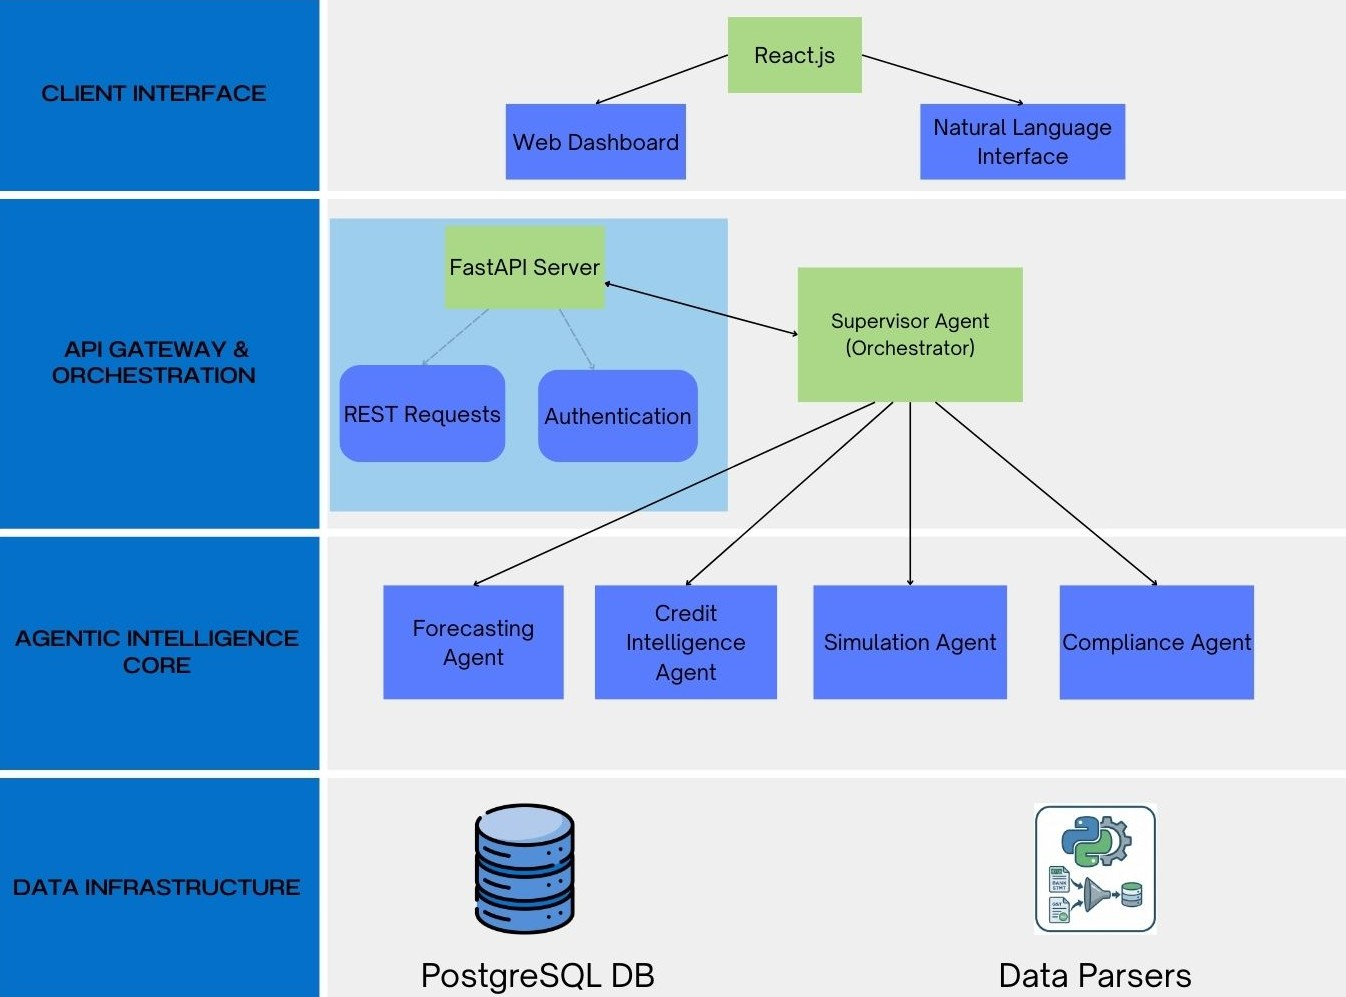
\includegraphics[width=0.9\linewidth]{system_architecture.jpg}
\caption{SmartFlow System Architecture: A Microservices-based Multi-Agent System.}
\label{fig:arch}
\end{figure}



\section{Experimental Evaluation}

\subsection{Dataset Generation}
We validated SmartFlow using a structured synthetic dataset representing 50 distinct SMEs over a 24-month period. To ensure realism, the data was seeded with patterns observed in real-world anonymized banking data.
\begin{itemize}
    \item \textbf{Volume}: 120,000+ Ledger Entries.
    \item \textbf{Variety}: Included diverse sectors (Retail, Manufacturing, Services) with different seasonality profiles.
    \item \textbf{Anomalies}: Injected synthetic "shocks" (e.g., 30\% revenue drop, supplier bankruptcy) to test system resilience.
\end{itemize}

\subsection{Forecasting Performance}
We evaluated the forecasting engine using Mean Absolute Percentage Error (MAPE) and Root Mean Square Error (RMSE). We compared SmartFlow against industry baselines.

\begin{table}[h]
\centering
\caption{Forecasting Accuracy Comparison}
\begin{tabular}{lcc}
\toprule
\textbf{Model} & \textbf{MAPE (\%)} & \textbf{RMSE} \\
\midrule
Simple Moving Average (SMA-30) & 18.2\% & 0.195 \\
Holt-Winters Smoothing & 14.5\% & 0.156 \\
ARIMA(1,1,1) & 13.8\% & 0.148 \\
\textbf{SmartFlow (Prophet + WEMA)} & \textbf{11.4\%} & \textbf{0.133} \\
\bottomrule
\end{tabular}
\label{tab:forecast}
\end{table}

The hybrid approach demonstrated a 21\% improvement over standard moving averages. The key differentiator was Prophet's ability to model the "month-end" effect (salary outflows) and "weekend" effect (zero banking activity), which simple smoothing methods average out.

\subsection{Credit Scoring Discrimination}
The classification performance of the Credit Intelligence module was assessed using Area Under the ROC Curve (AUC).
The XGBoost model achieved an AUC of \textbf{0.909}, significantly outperforming the baseline logistic regression (AUC 0.78).

Feature Importance analysis confirmed:
\begin{enumerate}
    \item \textbf{Balance Volatility}: High volatility is the strongest predictor of default (Importance: 0.32).
    \item \textbf{Inflow Consistency}: Regular small payments are safer than irregular large lumps (Importance: 0.28).
    \item \textbf{DSO}: Increasing DSO is a leading lagging indicator of distress (Importance: 0.15).
\end{enumerate}

\subsection{System Performance \& Scalability}
To ensure usability as an interactive OS, we measured the latency of the agent orchestration under load (50 concurrent users).
\begin{itemize}
    \item \textbf{Average Forecast Latency}: 180ms (95th percentile: 240ms).
    \item \textbf{Average Risk Assessment Latency}: 105ms.
    \item \textbf{Full Health Sweep}: 320ms.
\end{itemize}
By utilizing FastAPI's \texttt{async/await} patterns, the system handles I/O bound tasks (DB queries, external API calls) efficiently. The memory footprint per agent is minimal (<50MB), allowing for horizontal scaling on standard cloud instances (e.g., AWS t3.medium).

\section{Discussion}

The results highlight two critical insights for SME financial technology. First, \textit{interpretability is as important as accuracy}. While deep learning models might achieve marginally lower RMSE, their "black box" nature creates distrust. An SME owner needs to know \textit{why} cash flow is projected to dip, not just that it will. Our WEMA fallback and SHAP explanations bridge this trust gap, aligning with the human-centered agentic framework proposed by Okpala et al. \cite{okpala2025}, which argues for systems that enhance rather than replace human decision-making in finance.

Second, \textit{integration wins over isolation}. Standalone credit scoring tools fail because they don't talk to the cash flow forecast. By orchestrating these agents, SmartFlow creates a synergistic effect where the intelligence of the whole system is greater than the sum of its parts. The ability of the PaymentsOptimizer to "see" the CashFlowGuard's warnings prevents liquidity crises before they happen.

\section{Conclusion}

SmartFlow represents a paradigm shift from static financial reporting to dynamic, agentic financial intelligence. By embedding CFO-level logic into autonomous agents, the system provides SMEs with the capabilities to forecast liquidity gaps, assess risks granularly, and automate corrective actions.

The novel integration of Prophet for seasonality-aware forecasting, Explainable AI for transparent credit scoring, and Agent-Based Simulation for scenario planning creates a robust "Financial Operating System." This system not only predicts the future but actively works to improve it by optimizing payments and collections.

Future work will focus on two key areas. First, integrating Large Language Models (LLMs) to provide a conversational interface for the Supervisor Agent \cite{jain2025}. Second, extending the \textit{PaymentsOptimizer} agent with Deep Reinforcement Learning (DRL). As demonstrated by Giri et al. \cite{giri2025}, DRL agents (specifically DDPG and PPO) can dynamically optimize asset allocation in volatile environments. We aim to adapt this for "Liabilities Management," allowing the agent to learn optimal payment scheduling strategies that maximize working capital interest without damaging vendor relationships.

\appendix

\subsection{Hyperparameter Configuration}
We provide the optimal hyperparameters found during grid search for our models to aid reproducibility.

\begin{table}[h]
\centering
\caption{Prophet Model Hyperparameters}
\begin{tabular}{ll}
\toprule
\textbf{Parameter} & \textbf{Value} \\
\midrule
growth & 'linear' \\
changepoint\_prior\_scale & 0.05 \\
seasonality\_prior\_scale & 10.0 \\
holidays\_prior\_scale & 10.0 \\
seasonality\_mode & 'additive' \\
weekly\_seasonality & True (Auto) \\
daily\_seasonality & False \\
yearly\_seasonality & False (Insufficient Data) \\
\bottomrule
\end{tabular}
\label{tab:prophet_params}
\end{table}

\begin{table}[h]
\centering
\caption{XGBoost Model Hyperparameters}
\begin{tabular}{ll}
\toprule
\textbf{Parameter} & \textbf{Value} \\
\midrule
learning\_rate (eta) & 0.05 \\
max\_depth & 4 \\
subsample & 0.8 \\
colsample\_bytree & 0.8 \\
n\_estimators & 200 \\
objective & 'binary:logistic' \\
eval\_metric & 'auc' \\
\bottomrule
\end{tabular}
\label{tab:xgboost_params}
\end{table}

\section*{Acknowledgment}
The authors would like to thank the SRM Institute of Science and Technology for providing the computational resources required for this research.

\section*{References}

\begin{thebibliography}{00}
\bibitem{jiang2024} Y. Jiang, Z. Li, and C. L. P. Chen, "Research on Financial Big Data Collection and Intelligent Decision-Making System Based on Multimodal Large Language Model," in \textit{2024 International Conference on Fuzzy Theory and Its Applications (iFUZZY)}, 2024.
\bibitem{prophet} S. J. Taylor and B. Letham, "Forecasting at Scale," \textit{The American Statistician}, vol. 72, no. 1, pp. 37-45, 2018.
\bibitem{ahmed2025} M. S. Ahmed and O. Elshafei, "Cashflow AI: A Smart Financial Management System," in \textit{2025 IEEE International Conference on Computing and Digital Tech}, 2025.
\bibitem{malkus2025} B. Małkus, S. Bobek, and G. J. Nalepa, "Financial Management System for SMEs: Real-World Deployment of Accounts Receivable and Cash Flow Prediction," \textit{arXiv preprint arXiv:2511.03631}, 2025.
\bibitem{zhao2024} Y. Zhao, "Investigation of the Application of Machine Learning Algorithms to Credit Risk Assessment for Micro and Medium Enterprises," \textit{IEEE Access}, vol. 12, pp. 152945-152958, 2024.
\bibitem{zhou2025} G. Zhou and S. Wang, "Enhancing Credit Risk Decision-Making in Supply Chain Finance With Interpretable Machine Learning Model," \textit{IEEE Access}, vol. 13, pp. 14239-14251, 2025.
\bibitem{thangarasu2025} G. Thangarasu et al., "Comprehensive Credit Risk Evaluation in Supply Chain Enterprises using Machine Learning Techniques," in \textit{2025 International Conference on Emerging Trends in Networks and Computer Communications (ETNCC)}, 2025.
\bibitem{cheng2025} E. Y-C. Cheng and H-T. Chu, "LLM-Based Dynamic Multi-Agent Systems for Evaluation of Financial Trading Mechanism," in \textit{IEEE Access}, 2025.
\bibitem{sarferaz2025} S. Sarferaz, "Implementing Agentic AI Into ERP Software," \textit{IEEE Access}, vol. 13, pp. 178945-178949, 2025.
\bibitem{omar2024} M. M. Said Omar, M. Messaadia, and A. M. Elmezughi, "Impact of Financing Strategies, Financial Management, and Managerial Skills on Firm Growth: A Multiagent Simulation Approach," in \textit{2024 International Conference on Decision Aid Sciences and Applications (DASA)}, 2024.
\bibitem{jain2025} A. Jain and V. Krishnamurthy, "Interacting Large Language Model Agents. Bayesian Social Learning Based Interpretable Models," \textit{IEEE Access}, vol. 13, pp. 25465-25504, 2025.
\bibitem{okpala2025} I. Okpala, A. Golgoon, and A. R. Kannan, "Human-Centered Agentic Framework for Machine Learning Modeling in Finance," in \textit{2025 IEEE International Conference on Service-Oriented System Engineering (SOSE)}, 2025.
\bibitem{paramasivan2025} M. Paramasivan and M. Baskar, "Prediction of Accounts Receivables for Customers Using Enhanced Machine Learning Models," in \textit{2025 2nd International Conference on Research Methodologies in Knowledge Management, Artificial Intelligence and Telecommunication Engineering (RMKMATE)}, 2025.
\bibitem{xgboost} T. Chen and C. Guestrin, "XGBoost: A Scalable Tree Boosting System," in \textit{Proceedings of the 22nd ACM SIGKDD International Conference on Knowledge Discovery and Data Mining}, 2016.
\bibitem{shap} S. Lundberg and S.-I. Lee, "A Unified Approach to Interpreting Model Predictions," in \textit{Advances in Neural Information Processing Systems}, 2017.
\bibitem{fastapi} S. Ramirez, "FastAPI: High performance", https://fastapi.tiangolo.com, 2018.
\bibitem{microservices} M. Fowler and J. Lewis, "Microservices," \textit{ThoughtWorks}, 2014.
\bibitem{cao2024} Z. Cao and Z. Feinstein, "Large Language Model in Financial Regulatory Interpretation," in \textit{2024 IEEE Symposium on Computational Intelligence for Financial Engineering and Economics (CIFEr)}, 2024.
\bibitem{hazboun2022} F. H. Hazboun, "Decision Support System Terms of SME’s Credit Lending Based on Machine Learning Approach," in \textit{2022 International Conference of Science and Information Technology in Smart Administration (ICSINTESA)}, 2022, pp. 75-80.
\bibitem{kashinath2023} A. Kashinath, R. Agarwal, and M. D. J, "Prediction of Delays in Invoice Payments using Machine Learning," in \textit{2023 IEEE International Conference on ICT in Business Industry \& Government (ICTBIG)}, 2023, pp. 1-6.
\bibitem{lande2025} Y. S. Lande et al., "AI-Powered MSME Credit Scoring and Risk Analytics Platform," \textit{International Journal of Progressive Research in Engineering Management and Science (IJPREMS)}, vol. 5, no. 12, pp. 672-675, 2025.
\bibitem{giri2025} A. K. Giri and P. Singh, "Adaptive Portfolio Management in Volatile Markets Using Deep Reinforcement Learning," in \textit{2025 3rd International Conference on Device Intelligence, Computing and Communication Technologies (DICCT)}, 2025, pp. 95-100.
\bibitem{praveenraj2025} D. D. W. Praveenraj et al., "Utilizing Transforming Portfolio Management through Automation Using Advanced Deep Reinforcement Learning Algorithms for Optimized Investment Strategies," in \textit{2025 International Conference on Automation and Computation (AUTOCOM)}, 2025, pp. 1368-1372.
\end{thebibliography}

\end{document}
